\chapter{Implémentation}
\section{Transformation CAN/CNA}
Afin de réalisé notre commande, nous avons dût transformer la valeur entière lue pour $V_S$ par le CAN en un équivalent de la tension de type nombre à virgule flottante. Nous avons réalisé cette transformation avec l'équation \ref{equ:CAN}. Figure \ref{fig:CAN_p}, nous pouvons observer les valeurs que peut convertir le CAN et les valeurs dont nous avons besoins. Ici, la plage de conversion est à moitié entièrement utilisée. 
\begin{LARGE}
Refaire l'eq. err !! 
\end{LARGE}
\begin{equation}
\label{equ:CAN}
V_{volt} = 
\left\lfloor 
\frac{2^{11}-1}{5}V_{CAN} +2^{11}
\right\rfloor
= 
\left\lfloor 
819*V_{CAN} + 2048
\right\rfloor
\end{equation}
En pratique, nous ferrons un et logique avec 
La génération de la sortie $V_M$ nécessite aussi une conversion du CNA depuis la tension calculée par la commande (nombre à virgule flottante) vers un entier compris entre $-5$ et $5$ Volts. Néanmoins, la commande calcule une valeur comprise entre $-5$ et $5$ Volts, mais la carte de puissance branchée sur la sortie du CNA nécessite en entrée une tension comprise entre $0$ et $5$ Volt. Il faut donc, dans un premier temps, redresser la valeur calculée $V_{com}$ par la sortie sur une intervalle $\left[0;5\right]$ $V_{redr}$, puis le convertir en entier $V_{CNA}$. Pour cela nous utilisons les équations suivantes :
\begin{equation}
\begin{array}{lcl}
V_{red}	&=&	\frac{1}{2}V_{com}+2,5\\
V_{CNA} &=& \frac{10}{2^{12}-1}V_{red}-5\\
V_{CNA} &=& \frac{V_{com}}{819} - \frac{4090}{819}
\end{array}
\end{equation}
\begin{figure}[!ht]%
\begin{minipage}{.5\textwidth}%
\centering
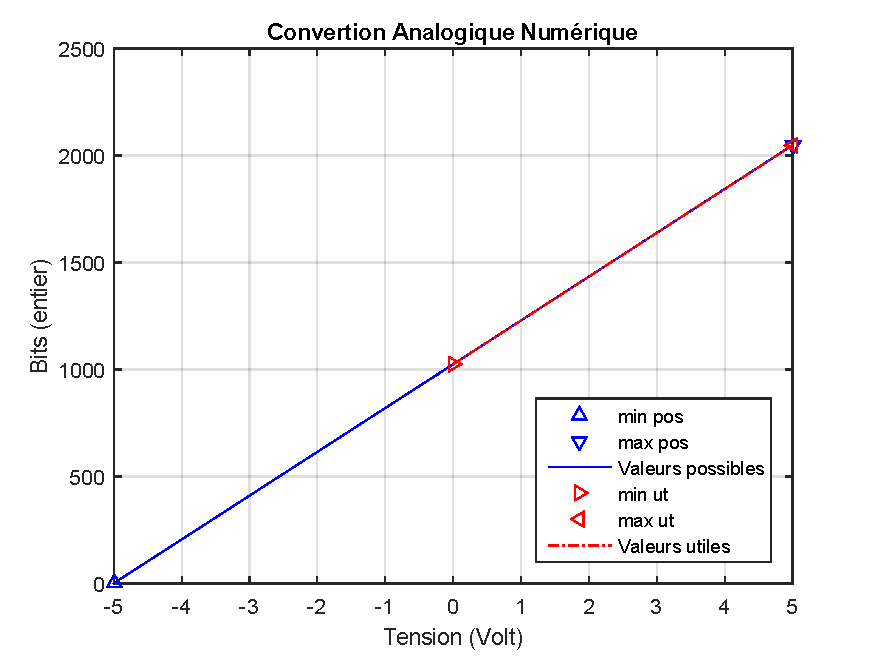
\includegraphics[width=\textwidth]{./VI/images/CAN_plage.pdf}
\caption{\label{fig:CAN_p}Valeurs possibles et possibles du CAN}
\end{minipage}%
\hfill%
\begin{minipage}{.5\textwidth}%
\centering
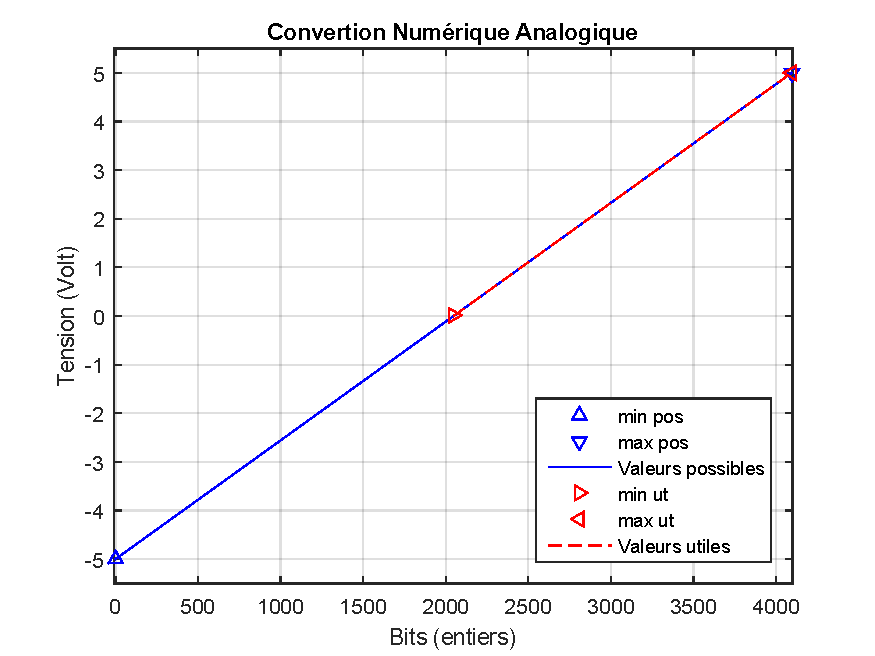
\includegraphics[width=\textwidth]{./VI/images/CNA_plage.pdf}
\caption{\label{fig:CNA_p}Valeurs possibles et possibles du CNA}
\end{minipage}%
\end{figure}
\begin{LARGE}
Erreur sur le nombre de bit CAN, vérifié le chap précédent aussi.
\end{LARGE}
%	\subsection{Implémentation d'un programme de test des convertisseurs}
%	\subsection{Correction}
	\subsection{Validation}
\section{Implémentation}
		\subsection{Description des taches}
		\subsection{implémentation}
		\subsection{Validation et correction}